\documentclass[a4paper,12pt]{article}

\usepackage[utf8]{inputenc}
\usepackage{parskip}
\usepackage[ngerman]{babel}
\usepackage{graphicx}

\title{OOAD Übungsblatt 3}
\author{Dominik Tödling, Lukas Neuhold, Christoph Huber,\\ Stefan Mitterrutzner, Emanuel Moser}

\begin{document}
\maketitle
\newpage
\part*{Abgabe 1}
\section*{Relationales Schema}
\textbf{foerdergeber} (\underline{foerdID}, name, addresse)\\
\textbf{foerdergeber\_telno} (\textit{\underline{foerdID}}, \underline{telno})\\
\textbf{projekt} (\underline{projektID}, name, startdatum, enddatum)\\
\textbf{industrieforschungsprojekt} (\textit{\underline{projektID}}, deckungsbeitrag)\\
\textbf{Grunlagenforschungsprojekt} (\textit{\underline{projektID}}, ausschreibungsakzeptanzrate)\\
\textbf{foerdert} (\textit{\underline{foerdID}, \underline{projektID}})\\
\textbf{partnerfirma} (\underline{partnerID}, name, addresse)\\
\textbf{ist\_zugeordnet} (\textit{\underline{industrieprojektID}, \underline{partnerID}}) \\
\textbf{mitarbeiter} (\underline{manr}, name)\\
\textbf{arbeitet\_in\_projekt} (\underline{id}, \textit{projektID, manr}, von, bis) \\
\textbf{abteilung} (\underline{abtnr}, name, \textit{manr}) \\
\textbf{arbeitet\_in\_abteilung} (\underline{id}, \textit{abtnr, manr}, von, bis) \\
\newpage
\part*{Abgabe 2}
\section*{Business Case}
IntelliCourse ist eine Software zur Zeitplanung von Kursen. Durch die automatische Zeitplanerstellung kann sich jeder ganz einfach seinen eigenen Zeitplan einsehen. Ein jeder User kann einen individualisierten Kalender mit allen Terminen ganz einfach einsehen.  Beim erstellen eines Events wird automatisch auf Zeit- und Raumüberschneidungen überprüft, und gegebenenfalls ein Warning ausgegeben, und es wird automatisch versucht alles so anzupassen, dass es zu keiner Überschneidung kommt. Durch diese automatisierte Einteilung von Terminen auf mögliche Räume und Timeslots wird sich viel an administrativem Aufwand erspart, was ermöglicht die Kosten in der Administration zu senken.Zusätzlich ist es möglich das  LehrendeZeitpräferenzen einzugeben, die in die Erstellung des Zeitplans miteinbezogen werden. Im falle dass ein Termin zu einem bestimmten Zeitpunkt stattfinden MUSS, kann ein Administrator den Zeitplan immer manuel bearbeiten.
\section*{Use Cases}
	\subsection*{Priorisierung und Szenarien}
	\begin{tabular}{|p{3cm}|c|p{3cm}|c|p{3cm}|c|}
		\hline
		\textbf{Student} & \textbf{Score} & \textbf{Lehrender} & \textbf{Score} & \textbf{Admin} & \textbf{Score} \\ \hline
		Anmelden & 10 & Anmelden & 10 & Anmelden & 10 \\ \hline
		Für Veranstaltung registrieren & 10 & Für Veranstaltung registrieren & 10 & Account erstellen & 10 \\ \hline
		Account erstellen & 10 & Account erstellen & 10 & Accounts authorisieren & 10 \\ \hline
		Kalender einsehen & 9 & Prüfung erstellen & 10 & Raum erstellen &  10 \\ \hline
		Event erstellen & 9 & Kurs erstellen & 10 & Für Veranstaltung registrieren  & 10  \\ \hline
		Event löschen & 9 & Kalender einsehen & 9 & Kurs erstellen & 10 \\ \hline
		&& Prüfung löschen & 9 & Prüfung erstellen & 10 \\ \hline
		&& Kurs löschen & 9 & Event erstellen & 9 \\ \hline
		&& Event löschen & 9 & Event löschen & 9 \\ \hline
		&&&& Kurs löschen & 9 \\ \hline
		&&&& Prüfung löschen & 9 \\ \hline
		&&&& Raum löschen & 9 \\ \hline
		&&&& Kalender einsehen & 9 \\ \hline
	\end{tabular}
	\newpage
	\subsection*{Use Case Spezifizierung}
	\begin{center}
		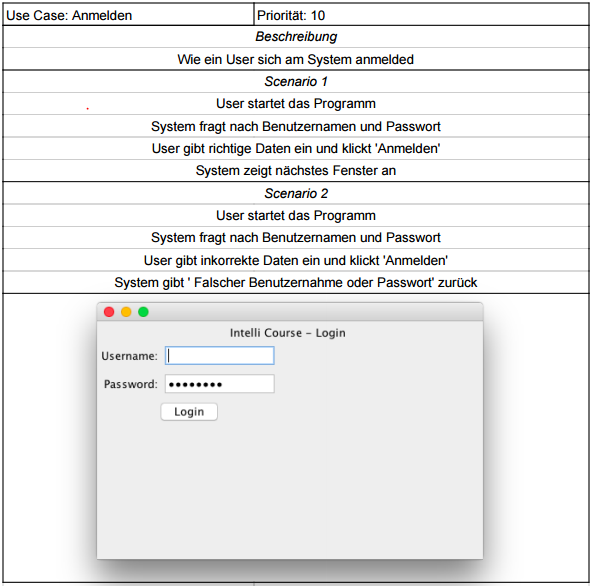
\includegraphics[scale=.8]{UCLogin.png}
		\newpage
		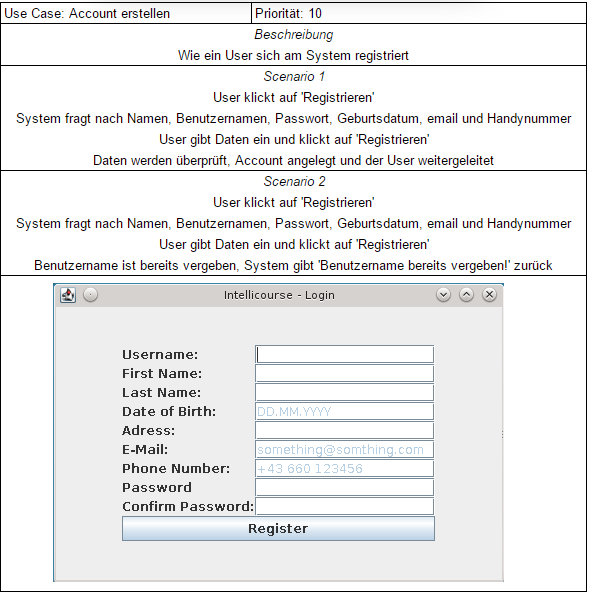
\includegraphics[scale=.8]{UCRegister.png}
		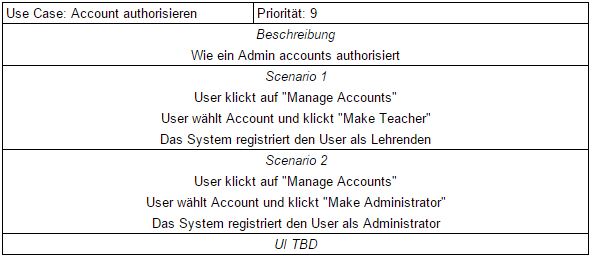
\includegraphics[scale=.8]{UCAuthorizeAccount.png}
		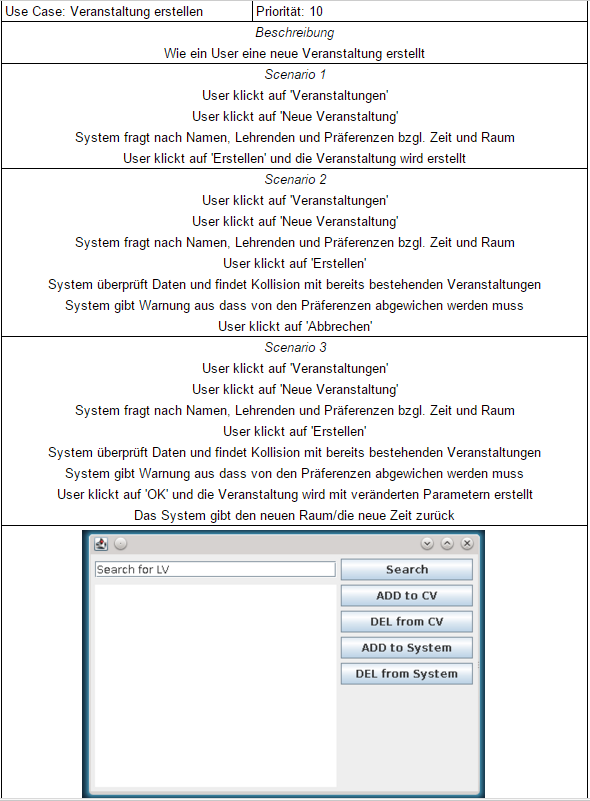
\includegraphics[scale=.8]{UCCreateHappening.png}
		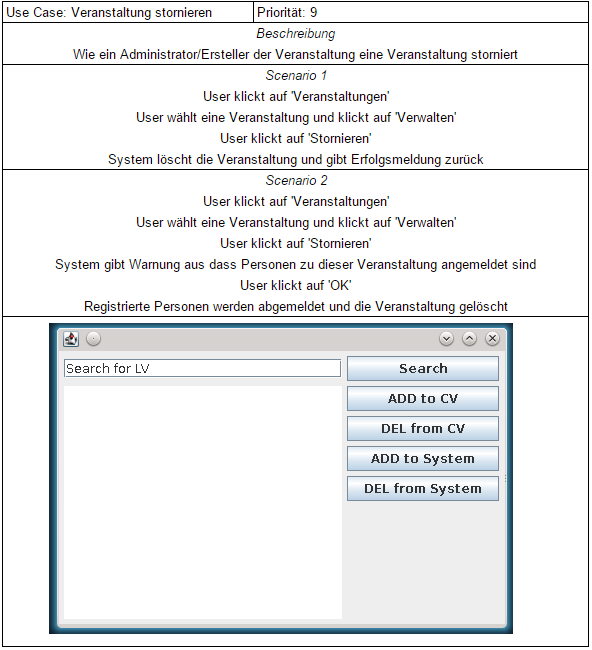
\includegraphics[scale=.8]{UCCancelHappening.png}
		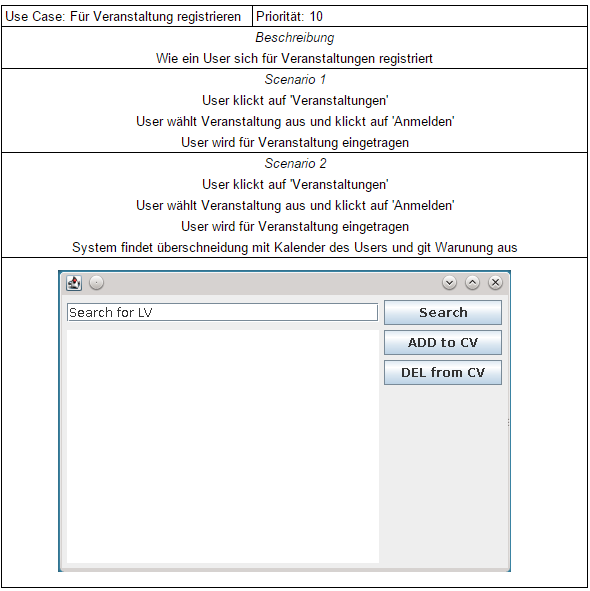
\includegraphics[scale=.8]{UCRegisterForHappening.png}
		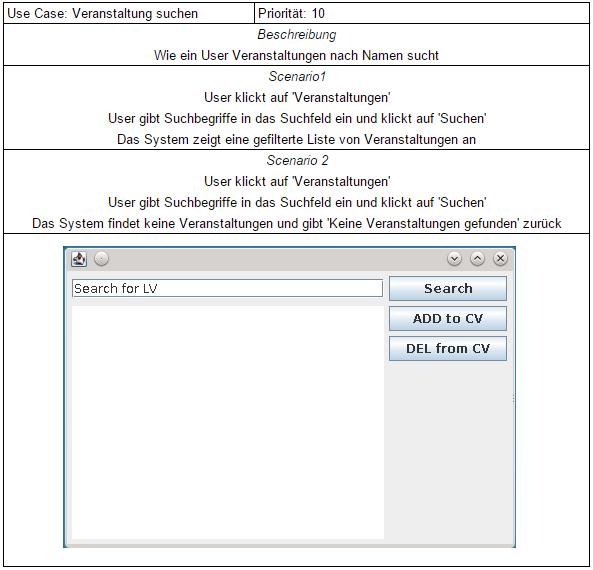
\includegraphics[scale=.8]{UCSearchHappening.png}
		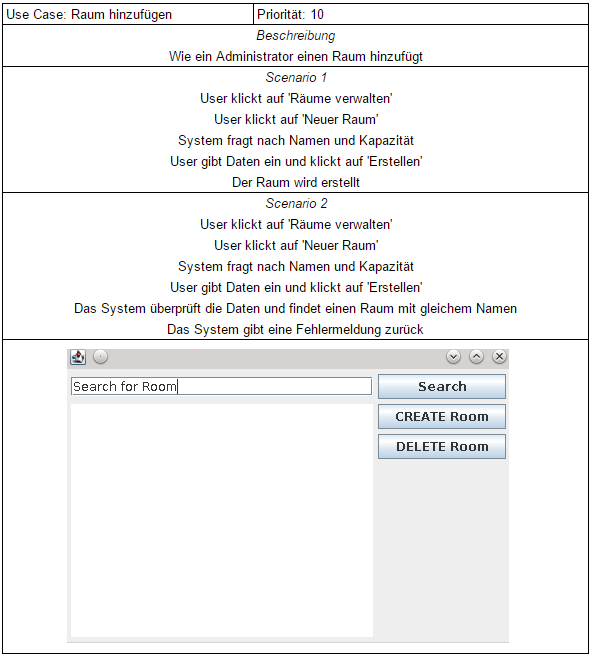
\includegraphics[scale=.8]{UCCreateRoom.png}
		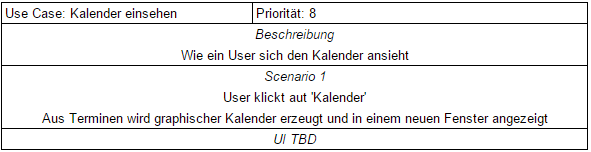
\includegraphics[scale=.8]{UCCalendar.png}
	\end{center}
	\subsection*{Use Case Diagramm}
	\begin{center}
		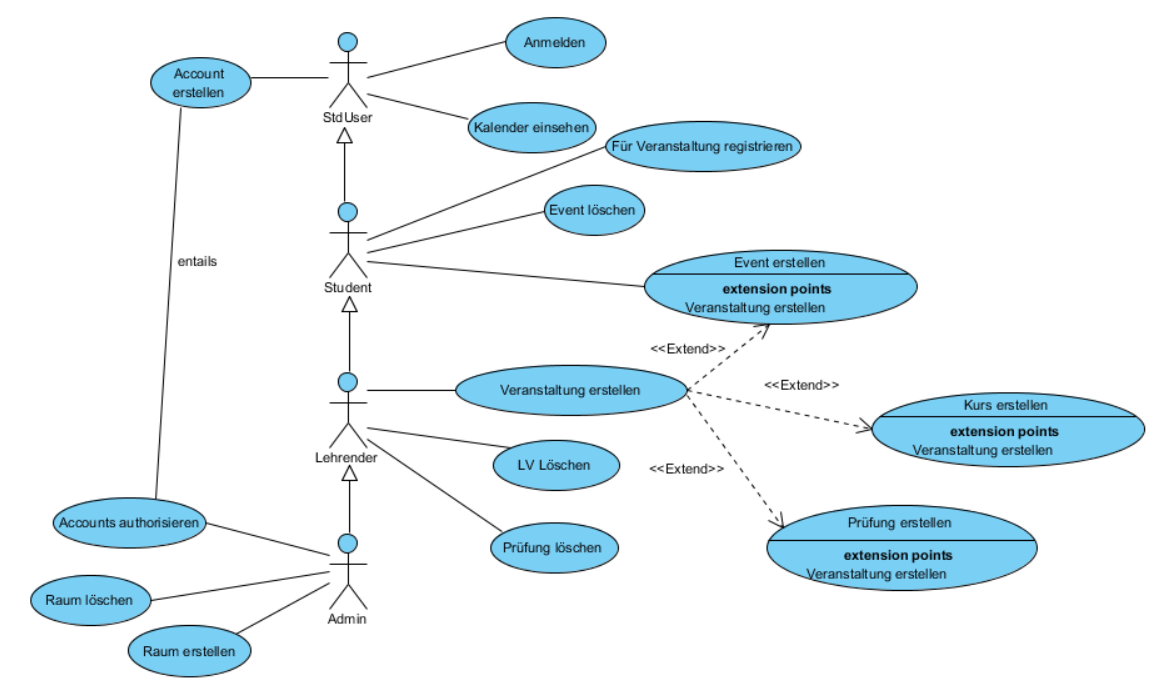
\includegraphics[scale=.5,angle=90]{UseCaseDiagram.png}
	\end{center}
	\subsection*{Sequenzdiagramme}
		\subsubsection*{Login}
			\begin{center}
				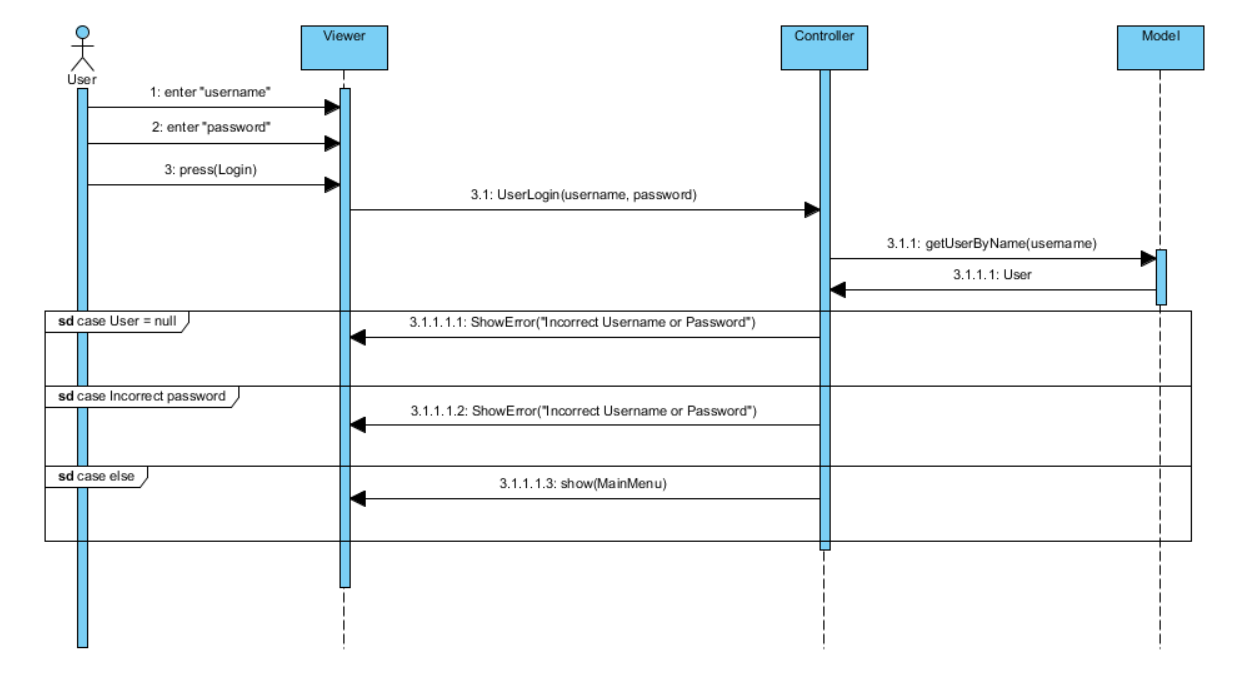
\includegraphics[scale=.5]{SeqLogin.png}
			\end{center}
		\subsubsection*{Registrieren}
			\begin{center}
				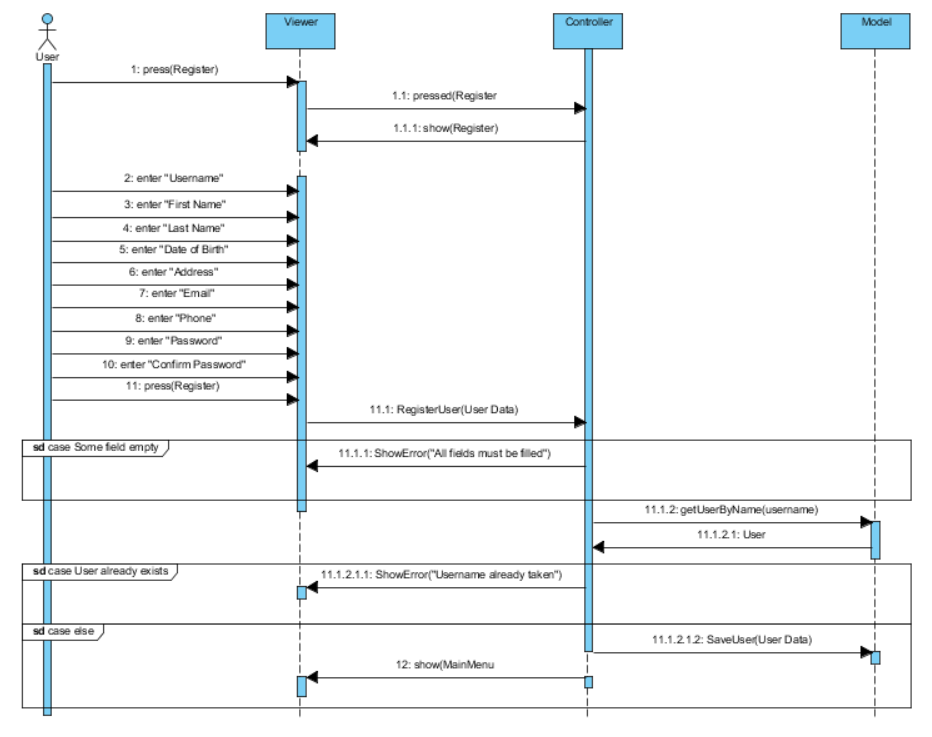
\includegraphics[scale=.5]{SeqRegister.png}
			\end{center}
		\subsubsection*{Raum erstellen}
			\begin{center}
				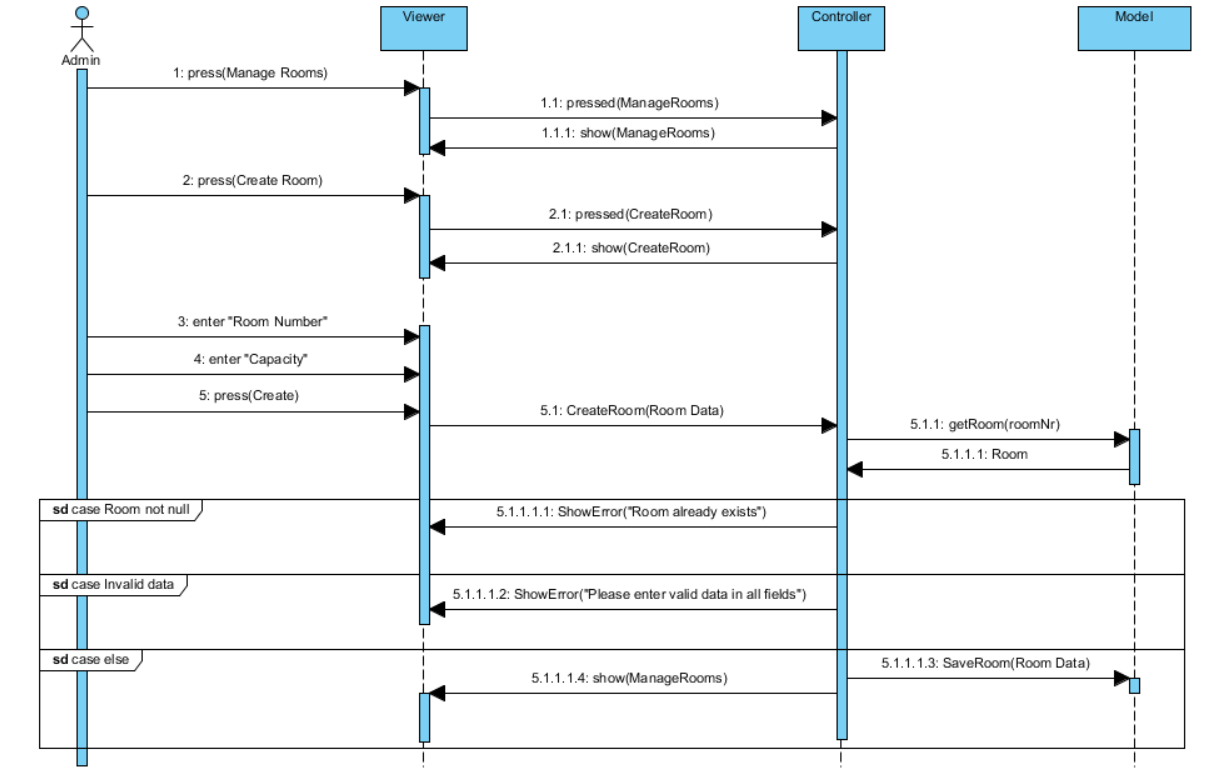
\includegraphics[scale=.5]{SeqCreateRoom.png}
			\end{center}
	\subsection*{State Machine Diagramme}
		\subsubsection*{Gesamtes Programm}
			\begin{center}
				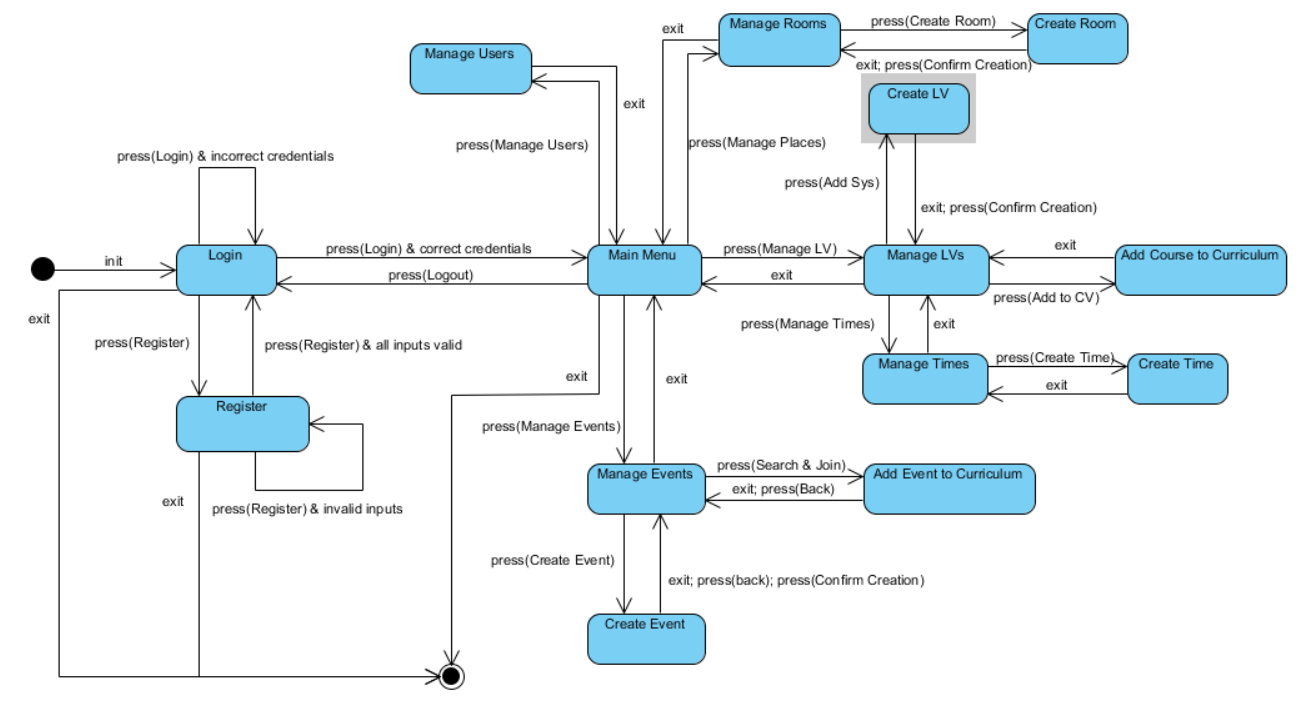
\includegraphics[scale=.5]{sc_all.png}
			\end{center}
		\subsubsection*{Login}
			\begin{center}
				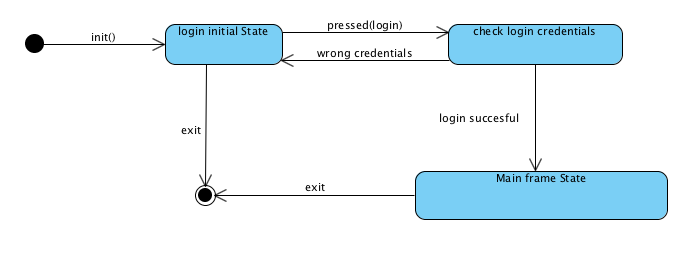
\includegraphics[scale=.5]{sc_login.png}
			\end{center}
		\subsubsection*{Registrieren}
			\begin{center}
				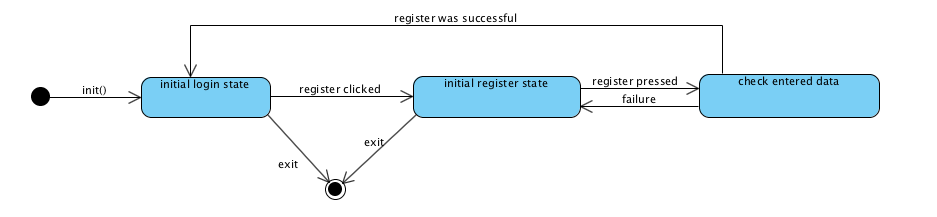
\includegraphics[scale=.5]{sc_register.png}
			\end{center}
		\subsubsection*{Raum erstellen}
			\begin{center}
				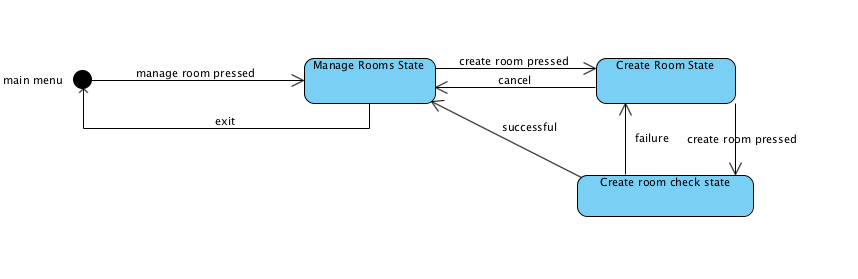
\includegraphics[scale=.5]{sc_manage_room.png}
			\end{center}
\section*{UML Analyse-Klassendiagramm}
\begin{center}
	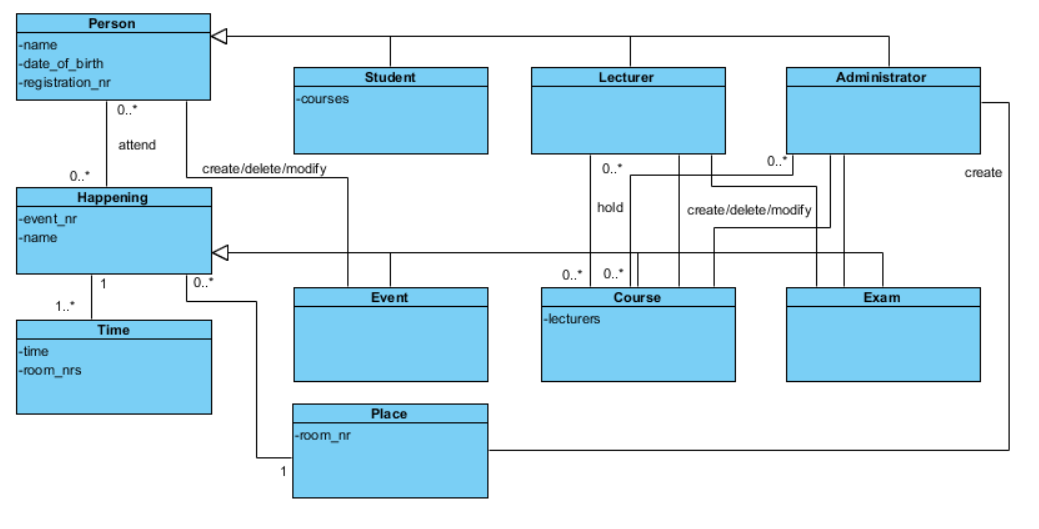
\includegraphics[scale=.7]{AnalysisClassDiagram.png}
\end{center}
\section*{UML Design-Klassendiagramm}
\begin{center}
	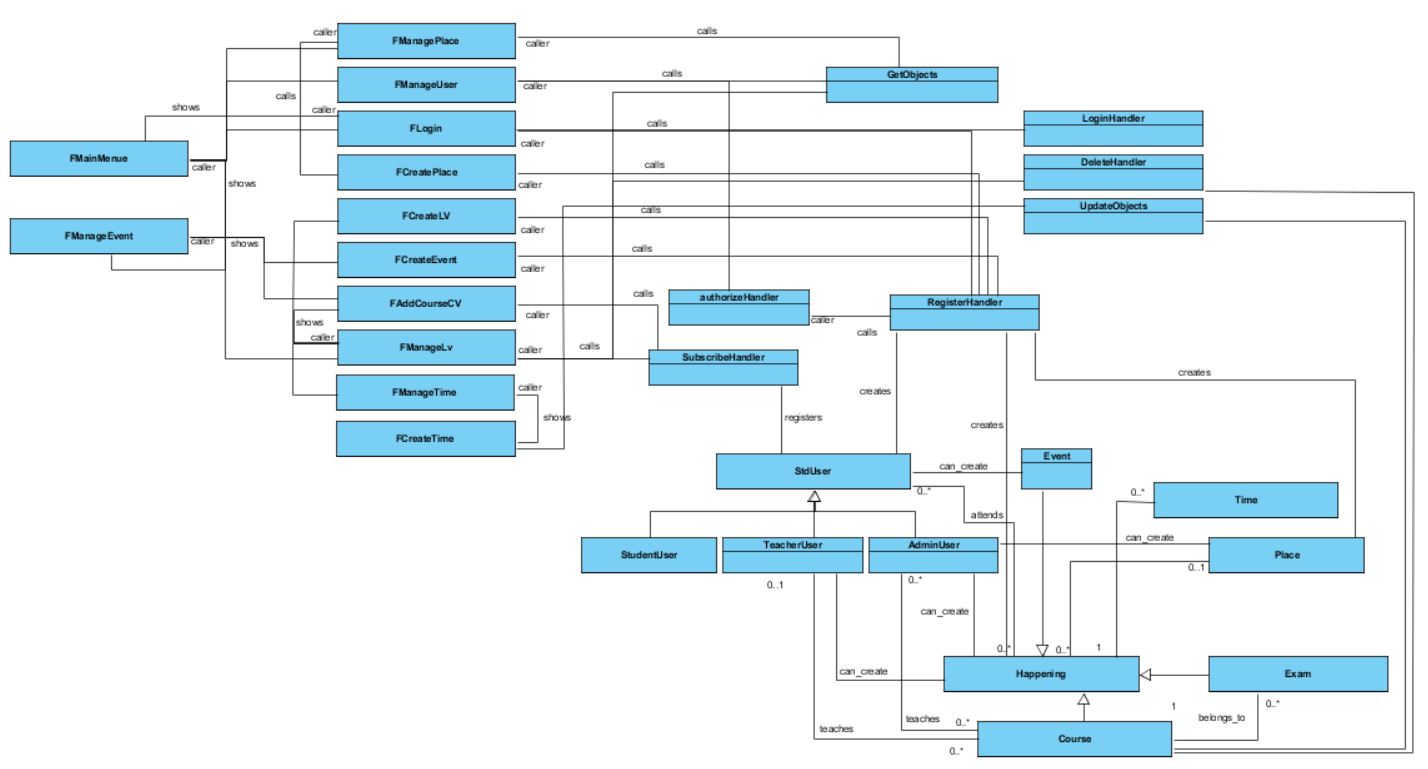
\includegraphics[scale=.7,angle=90]{DesignClassDiagram.png}
\end{center}
\subsection*{Einzelne Klassen}
Aus Gründen der Übersichtlichkeit wurden im obigen Diagramm die genauen Klassendefinitionen weggelassen und sind im folgenden zu sehen:
\begin{center}
	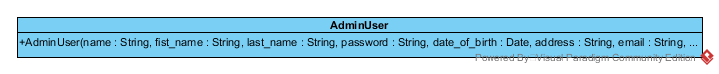
\includegraphics[scale=.8]{cAdminUser.png}
	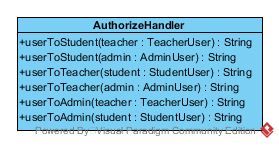
\includegraphics[scale=1]{cAuthorizeHandler.png}
	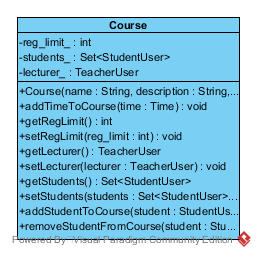
\includegraphics[scale=1]{cCourse.png}
	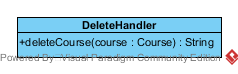
\includegraphics[scale=1]{cDeleteHandler.png}
	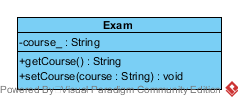
\includegraphics[scale=1]{cExam.png}
	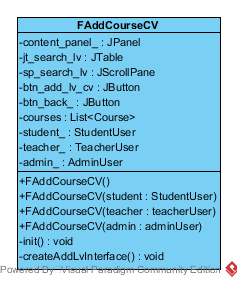
\includegraphics[scale=1]{cFAddCourseCV.png}
	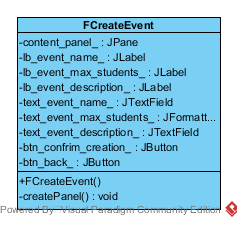
\includegraphics[scale=1]{cFCreateEvent.png}
	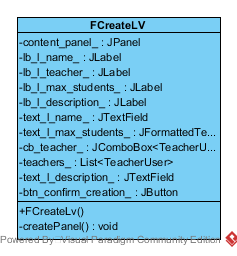
\includegraphics[scale=1]{cFCreateLv.png}
	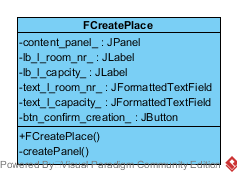
\includegraphics[scale=1]{cFCreatePlace.png}
	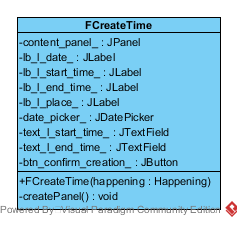
\includegraphics[scale=1]{cFCreateTime.png}
	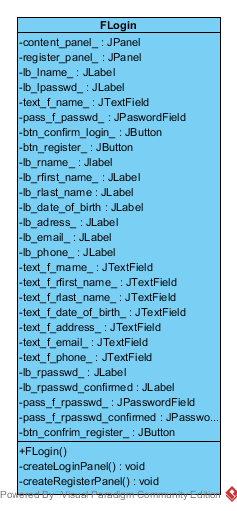
\includegraphics[scale=1]{cFLogin.png}
	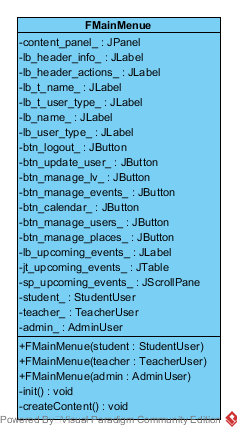
\includegraphics[scale=1]{cFMainMenue.png}
	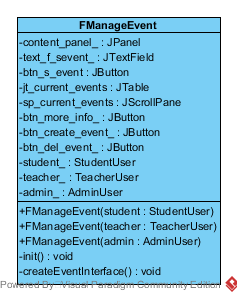
\includegraphics[scale=1]{cFManageEvent.png}
	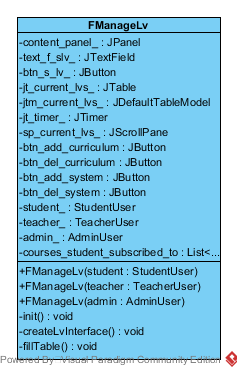
\includegraphics[scale=1]{cFManageLv.png}
	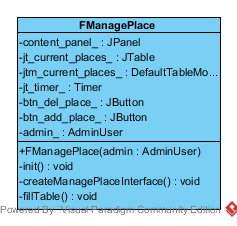
\includegraphics[scale=1]{cFManagePlace.png}
	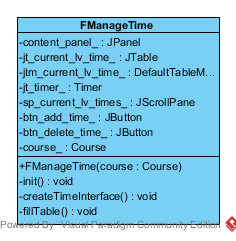
\includegraphics[scale=1]{cFManageTime.png}
	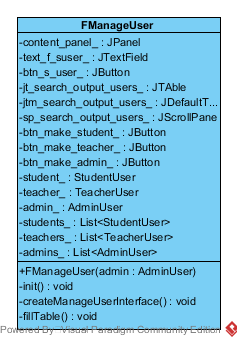
\includegraphics[scale=1]{cFManageUser.png}
	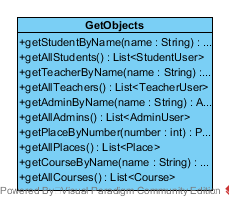
\includegraphics[scale=1]{cGetObjects.png}
	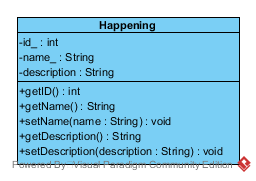
\includegraphics[scale=1]{cHappening.png}
	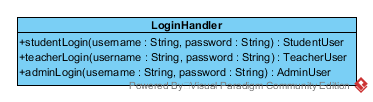
\includegraphics[scale=1]{cLoginHandler.png}
	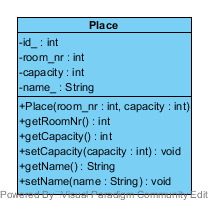
\includegraphics[scale=1]{cPlace.png}
	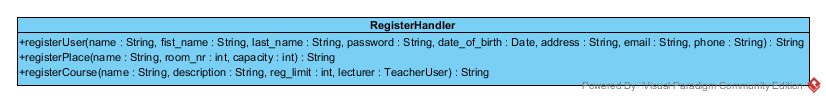
\includegraphics[scale=.8]{cRegisterHandler.png}
	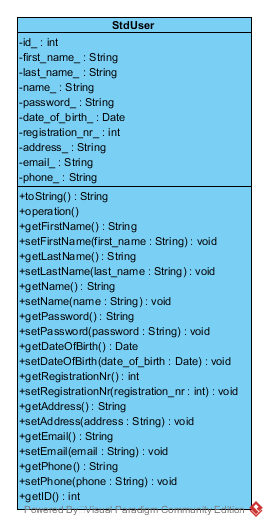
\includegraphics[scale=1]{cStdUser.png}
	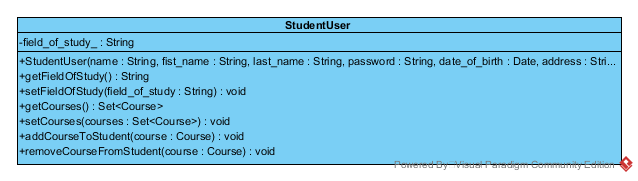
\includegraphics[scale=1]{cStudentUser.png}
	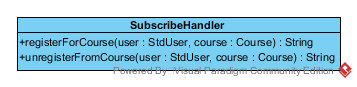
\includegraphics[scale=1]{cSubscribeHandler.png}
	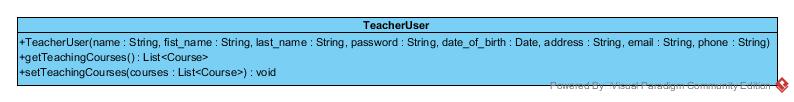
\includegraphics[scale=.8]{cTeacherUser.png}
	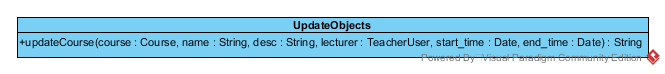
\includegraphics[scale=.9]{cUpdateObjects.png}
\end{center}
\newpage
\section*{Projektplan}
\begin{tabular}{|l|l|}
	\hline
	Accounts erstellen & fertig \\ \hline
	Räume erstellen & fertig \\ \hline
	Veranstaltungen erstellen & fertig \\ \hline
	Veranstaltung suchen & fertig \\ \hline
	Für Veranstaltungen registrieren/abmelden & fertig \\ \hline
	Berechtigungslevel für User & fertig \\ \hline
	Authorisierung von Usern & fertig \\ \hline
	Veranstaltungen suchen & fertig \\ \hline
	Manuelle verschiebung von Veranstaltungen & fertig \\ \hline
	Zeitplan einsehen & fertig \\ \hline
\end{tabular}
\section*{Projektbericht}
Unser Ziel mit diesem Projekt war es ein System zu entwickeln mit dem es möglich ist Kurse und Prüfungen, beziehungsweise Anmeldungen and diesen, einfach zu verwalten. Dabei mussten wir im Laufe der Entwicklung aufgrund von zeitlichen und technischen Problemen ein paar der höheren Ziele (wie etwa Zeitpräferenzen für Vortragende oder ein Semestersystem) weglassen und haben uns stattdessen auf die Grundfunktionalitäten fokusiert. \\
Die größten Probleme bei der Entwicklung wurden von der Datenbankanbindung ausgelöst und große Teile des Programmes mussten neu überarbeitet werden um bestimmte Fehler zu lösen. Erwähnenswert wäre hier zum Beispiel die Art und Weise wie Berechtigungslevel implementiert sind. Der Ursprüngliche Ansatz nutzte eine Vererbungskette, da ein Lehrender ja alles darf was ein Student darf usw. Dies verursachte jedoch beim Löschen und Suchen nach Personen einige Probleme und wurde im Endeffekt durch eine Einfache Vererbung ersetzt bei der jede der drei Klassen von einer gemeinsamen Klasse abgeleitet war.
\end{document}